\documentclass[11pt]{elegantbook}
\definecolor{structurecolor}{RGB}{40,58,129}
\linespread{1.6}
\setlength{\footskip}{20pt}
\setlength{\parindent}{0pt}
\newcommand{\argmax}{\operatornamewithlimits{argmax}}
\newcommand{\argmin}{\operatornamewithlimits{argmin}}
\elegantnewtheorem{proof}{Proof}{}{Proof}
\elegantnewtheorem{claim}{Claim}{prostyle}{Claim}
\DeclareMathOperator{\col}{col}
\title{\textbf{Economic Theory}}
\author{Wenxiao Yang}
\institute{Haas School of Business, University of California Berkeley}
\date{2023}
\setcounter{tocdepth}{2}
\cover{cover.png}
\extrainfo{All models are wrong, but some are useful.}

% modify the color in the middle of titlepage
\definecolor{customcolor}{RGB}{9,119,119}
\colorlet{coverlinecolor}{customcolor}
\usepackage{cprotect}

\addbibresource[location=local]{reference.bib} % bib

\begin{document}

\maketitle
\frontmatter
\tableofcontents
\mainmatter



\chapter{Signalling Game}
Based on
\begin{enumerate}[$\circ$]
    \item "Kreps, D. M., \& Sobel, J. (1994). Signalling. \textit{Handbook of game theory with economic applications}, 2, 849-867."
    \item 
\end{enumerate}

\section{Canonical Game}
\begin{definition}[Canonical Game]
    \normalfont
    \begin{enumerate}
        \item There are two players: $\mathbf{S}$ (sender) and $\mathbf{R}$ (receiver).
        \item $\mathbf{S}$ holds more information than $\mathbf{R}$: the value of some random variable $t$ with support $\mathcal{T}$. (We say that $t$ is the \textbf{type} of $\mathbf{S}$)
        \item Prior belief of $\mathbf{R}$ concerning $t$ are given by a probability distribution $\rho$ over $\mathcal{T}$ (common knowledge)
        \item $\mathbf{S}$ sends a \textbf{signal $s\in \mathcal{S}$} to $\mathbf{R}$ drawn from a signal set $\mathcal{S}$.
        \item $\mathbf{R}$ receives this signal, and then takes an \textbf{action} $a\in \mathcal{A}$ drawn from a set $\mathcal{A}$ (which could depend on the signal $s$ that is sent).
        \item $\mathbf{S}$'s payoff is given by a function $u: \mathcal{T}\times \mathcal{S} \times \mathcal{A} \rightarrow \mathbb{R}$ and $\mathbf{R}$'s payoff is given by a function $v: \mathcal{T}\times \mathcal{S} \times \mathcal{A} \rightarrow \mathbb{R}$.
    \end{enumerate}
\end{definition}

\section{Nash Equilibrium}
\begin{definition}[Strategy]
    \normalfont
    A \textbf{behavior strategy} for $\mathbf{S}$ is given by a function $\sigma: \mathcal{T}\times\mathcal{S} \rightarrow [0,1]$ such that $\sum_s \sigma(t,s)$ for each $t$.\\
    A \textbf{behavior strategy} for $\mathbf{R}$ is given by a function $\alpha: \mathcal{S}\times\mathcal{A} \rightarrow [0,1]$ such that $\sum_a \alpha(s,a)$ for each $t$.
\end{definition}

\begin{definition}[Nash Equilibrium]
    \normalfont
    Behavior strategies $\alpha$ and $\sigma$ form a \textbf{Nash equilibrium} if and only if
    \begin{enumerate}
        \item For all $t\in \mathcal{T}$,
        \begin{center}
            $\sigma(t,s)>0$ implies $\sum_a \alpha(s,a)u(t,s,a) = \max_{s'\in \mathcal{S}}\left(\sum_a \alpha(s',a)u(t,s',a)\right)$
        \end{center}
        \item For each $s\in \mathcal{S}$ such that $\sum_{t}\sigma(t,s)\rho(t)>0$,
        \begin{center}
            $\alpha(s,a)>0$ implies $\sum_{t}\mu(t;s)v(t,s,a) = \max_{a'}\sum_{t}\mu(t;s)v(t,s,a')$
        \end{center}
        where $\mu(t;s)$ is the $\mathbb{R}$'s posterior belief about $t$ given $s$, $\mu(t;s)=\frac{\sigma(t,s)\rho(t)}{\sum_{t'}\sigma(t',s)\rho(t')}$ if $\sum_t\sigma(t,s)\rho(t)>0$ and $\mu(t;s)=0$ otherwise.
    \end{enumerate}
\end{definition}

\begin{definition}[Separating \& Pooling Equilibrium]
    \normalfont
    An equilibrium $(\sigma,\alpha)$ is called a \textbf{separating} equilibrium if each type $t$ sends different signals; i.e., the set $\mathcal{S}$ can be partitioned into (disjoint) sets $\{\mathcal{S}_t; t\in \mathcal{S}\}$ such that $\sigma(t, \mathcal{S}_t) = 1$. An equilibrium $(\sigma,\alpha)$ is called a \textbf{pooling} equilibrium if there is a single signal $s^*$ that is sent by all types; i.e., $\sigma(t, s^*) = 1$ for all $t\in \mathcal{T}$.
\end{definition}


\section{Single-crossing}

\subsection{Situation over real line}
Consider the situation that $\mathcal{T},\mathcal{S},\mathcal{A}\subseteq \mathbb{R}$ and $\geq$ is the usual "greater than or equal to" relationship.

\begin{enumerate}
    \item We let $\Delta \mathcal{A}$ denote the set of probability distributions on $\mathcal{A}$.
    \item For each $s\in \mathcal{S}$ and $\mathcal{T}'\subseteq \mathcal{T}$, we let $\Delta\mathcal{A}(s,T')$ be the set of mixed strategies that are the best responses by $\mathbf{R}$ to $s\in \mathcal{S}$ for some probability distribution with support $\mathcal{T}'$.
    \item For $\alpha\in \Delta\mathcal{A}$, we write $u(t,s,\alpha)\triangleq \sum_{a\in \mathcal{A}}u(t,s,a)\alpha(a)$.
\end{enumerate}

\begin{definition}[Single-crossing]
    \normalfont
    The data of the game are said to satisfy the \textbf{single-crossing property} if the following holds: If $t\in \mathcal{T}$, $(s,\alpha)\in \mathcal{S}\times \Delta\mathcal{A}$ and $(s',\alpha')\in \mathcal{S}\times \Delta\mathcal{A}$ are such that $\alpha\in \Delta\mathcal{A}(s,\mathcal{T})$, $\alpha'\in \Delta\mathcal{A}(s',\mathcal{T})$, $s>s'$ and $u(t,s,\alpha)\geq u(t,s',\alpha')$, then for all $t'\in T$ such that $t'>t$, $u(t',s,\alpha)\geq u(t',s',\alpha')$.
\end{definition}


\chapter{Stochastic Dominance}
Based on
\begin{enumerate}[$\circ$]
    \item MIT 14.123 S15 Stochastic Dominance Lecture Notes
    \item Princeton ECO317 Economics of Uncertainty Fall Term 2007 Notes for lectures 4. Stochastic Dominance
\end{enumerate}

\section{First-order Stochastic Dominance}
\subsection{Two Equivalent Definitions}
\begin{definition}[First-order Stochastic Dominance]
    \normalfont
    For any lotteries $F$ and $G$, $F$ \textbf{first-order stochastically dominates} $G$ if and only if the decision maker weakly prefers $F$ to $G$ under every \underline{weakly increasing} utility function $u$, i.e.,
    $$\int u (x) dF \geq \int u(x) dG$$
\end{definition}

\begin{definition}[First-order Stochastic Dominance]
    \normalfont
    For any lotteries $F$ and $G$, $F$ \textbf{first-order stochastically dominates} $G$ if and only if
    $$F(x)\leq G(x),\forall x$$
\end{definition}

\begin{center}\begin{figure}[htbp]
    \centering
    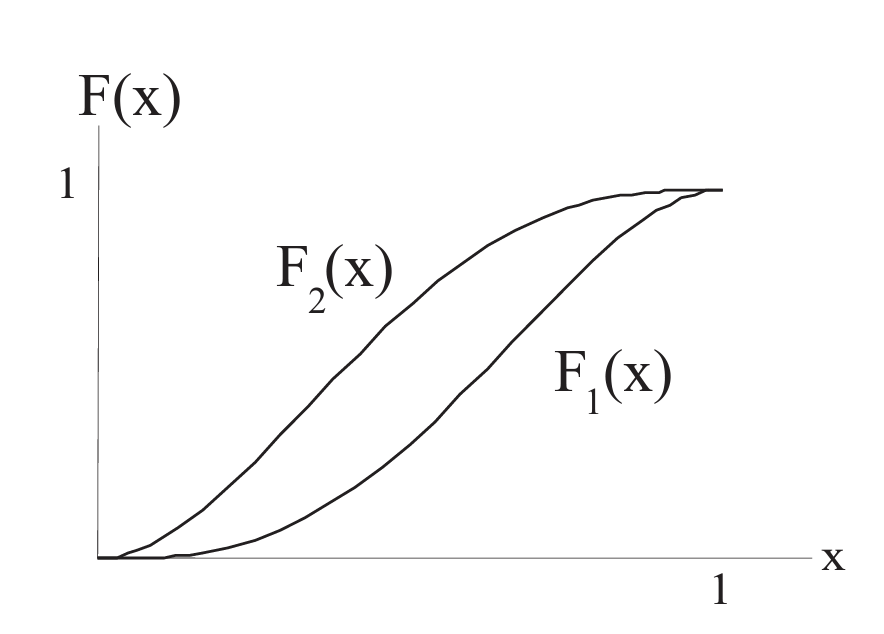
\includegraphics[scale=0.2]{FOSD_1.png}
    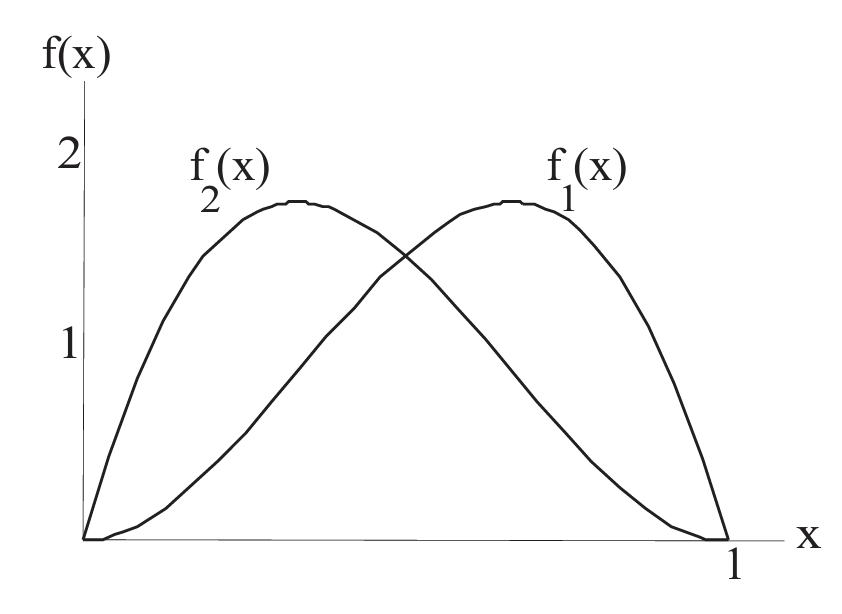
\includegraphics[scale=0.2]{FOSD_2.png}
    \caption{$F_1$ is FOSD over $F_2$: CDF and density comparison}
    \label{}
\end{figure}\end{center}

\section{Second-order Stochastic Dominance}
\subsection{Definition in terms of final goals}
\begin{definition}[Second-order Stochastic Dominance]
    \normalfont
    For any lotteries $F$ and $G$, $F$ \textbf{second-order stochastically dominates} $G$ if and only if the decision maker weakly prefers $F$ to $G$ under every \underline{weakly increasing \textbf{concave}} utility function $u$, i.e.,
    $$\int u (x) dF \geq \int u(x) dG$$
\end{definition}
\begin{center}\begin{figure}[htbp]
    \centering
    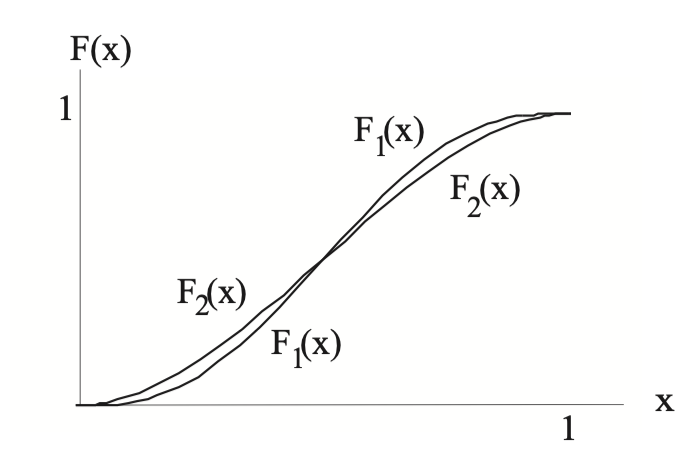
\includegraphics[scale=0.25]{SOSD_1.png}
    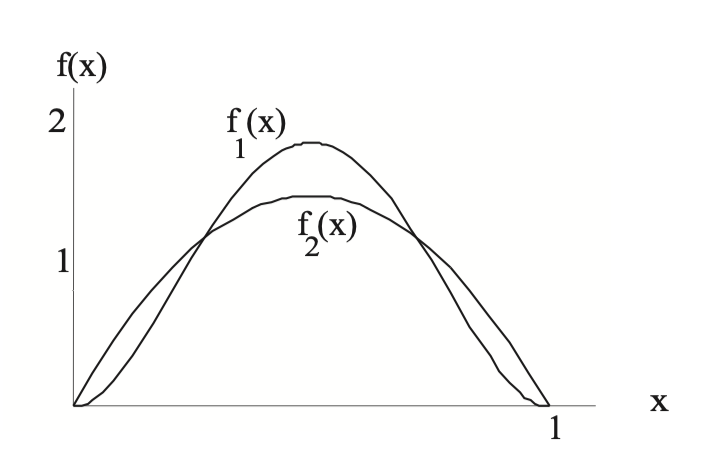
\includegraphics[scale=0.25]{SOSD_2.png}
    \caption{$F_1$ is SOSD over $F_2$: CDF and density comparison}
    \label{}
\end{figure}\end{center}

\subsection{Mean-Preserving Spread}
\begin{definition}[Mean-Preserving Spread]
    \normalfont
    Let $x_F$ and $x_G$ be the random variables associated with lotteries $F$ and $G$. Then $G$ is a \textbf{mean-preserving spread} of $F$ if and only if $$x_G \stackrel{d}{=} x_F+\varepsilon$$
    for some random variable $\varepsilon$ such that $\mathbb{E}(\varepsilon\mid x_F)=0,\forall x_F$.
\end{definition}
The "$\stackrel{d}{=}$" means "is equal in distribution to" (that is, "has the same distribution as").

\begin{note}
    Given $G$ is a \textbf{mean-preserving spread} of $F$, $G$ has larger variance than $F$.
\end{note}

\begin{example}
    $F(198)=\frac{1}{2}, F(202)=\frac{1}{2}$ and $G(100)=\frac{1}{100}$, $G(200)=\frac{98}{100}$, $G(300)=\frac{1}{100}$. Then $$x_G \stackrel{d}{=} x_F+\varepsilon$$
    where the distribution of $\varepsilon$ can be solved by $\left\{\begin{matrix}
        \frac{1}{100}&=\frac{1}{2}P(\varepsilon=102)+\frac{1}{2}P(\varepsilon=98)\\
        \frac{98}{100}&=\frac{1}{2}P(\varepsilon=2)+\frac{1}{2}P(\varepsilon=-2)\\
        \frac{1}{100}&=\frac{1}{2}P(\varepsilon=-98)+\frac{1}{2}P(\varepsilon=-102)
    \end{matrix}\right.$
\end{example}


\subsection{Second-order Stochastic Dominance is equivalent to Mean-Preserving Spread}
\begin{theorem}[Second-order Stochastic Dominance Equivalence]\label{SOSD_equiv}
    Given $\int x dF=\int x dG$ (same mean). The following are equivalent.
    \begin{enumerate}
        \item $F$ second-order stochastically dominates $G$: $\int u (x) dF \geq \int u(x) dG$  for every weakly increasing concave utility function $u$.
        \item $G$ is a mean-preserving spread of $F$.
        \item For every $t\geq 0$, $\int_a^t G(x)dx\geq \int_a^t F(x)dx$.
    \end{enumerate}
\end{theorem}
\begin{center}\begin{figure}[htbp]
    \centering
    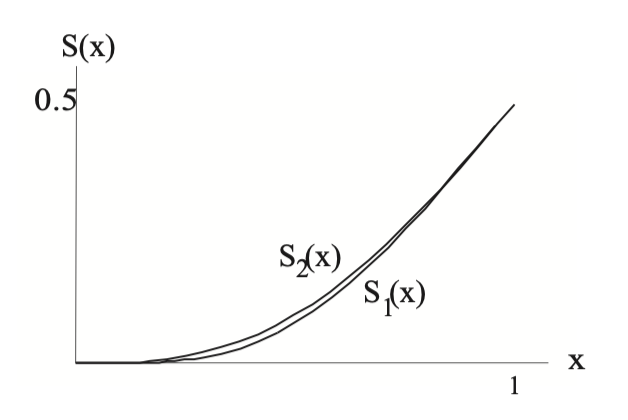
\includegraphics[scale=0.25]{SOSD_3.png}
    \caption{$F_1$ is SOSD over $F_2$, $S(t):\int_a^t F_2(x)dx\geq \int_a^t F_1(x)dx$}
    \label{}
\end{figure}\end{center}


















\chapter{Bayesian Persuasion: Useful Mathematical Results}
Based on
\begin{enumerate}[$\circ$]
    \item Kleiner, A., Moldovanu, B., \& Strack, P. (2021). Extreme points and majorization: Economic applications. \textit{Econometrica}, 89(4), 1557-1593.
    \item 
\end{enumerate}

\section{Majorization}
\subsection{Majorization and Weak Majorization}
\begin{definition}[Majorization]
    \normalfont
    Consider right-continuous functions that map the unit interval $[0,1]$ into the real numbers. For two \underline{non-decreasing} functions $f,g \in L^1$, we say that $f$ \textbf{majorizes} $g$, denoted by $g \prec f$, if the following two conditions hold:
    \begin{equation}
        \begin{aligned}
            \int_x^1 g(s)ds\leq \int_x^1 f(s)ds,\forall x\in [0,1]
        \end{aligned}
        \tag{Condition 1}
        \label{C1}
    \end{equation}
    \begin{equation}
        \begin{aligned}
            \int_0^1 g(s)ds=\int_0^1 f(s)ds
        \end{aligned}
        \tag{Condition 2}
        \label{C2}
    \end{equation}
\end{definition}

\begin{definition}[Weak Majorization]
    \normalfont
    $f$ \textbf{weakly majorizes} $g$, denoted by $g \prec_w f$, if \ref{C1} holds (not necessarily \ref{C2}).
\end{definition}

\subsection{How to work for non-monotonic functions? -- Non-Decreasing Rearrangement}
\begin{note}
    \normalfont
    \textbf{How this work with non-monotonic functions?}\\
    Suppose $f,g$ are non-monotonic, we compare their non-decreasing rearrangements $f^*$, $g^*$.
    \begin{definition}[Rearrangement]
        \normalfont
        Given a function $f$, let $m(x)$ denote the Lebesgue measure of the set $\{s \in[0, 1]: f(s)\leq x\}$, that is $m(x)=\int_{s\in\{s \in[0, 1]: f(s)\leq x\}}1ds$ (the "length" of the set). The non-decreasing rearrangement of $f$, $f^*$, is defined by $$f^*(t) = \inf\{ x \in \mathbb{R}: m(x) \geq t\},\ t\in[0,1]$$
    \end{definition}
\end{note}

\subsection{Generalized Inverse $G^{-1}(x)=\sup\{s:G(s)\leq x\}$}
\begin{definition}[Generalized Inverse]
    \normalfont
    Suppose $G$ is defined on the interval $[0,1]$, we can define the \textbf{generalized inverse}
    $$G^{-1}(x)=\sup\{s:G(s)\leq x\}, x\in [0,1]$$
\end{definition}

\subsection{Theorem: $F$ majorizes $G$ $\Leftrightarrow$ $G$ is a mean-preserving spread of $F$}
Based on
\begin{enumerate}[$\circ$]
    \item Shaked, M., \& Shanthikumar, J. G. (2007). \textit{Stochastic orders}. New York, NY: Springer New York.
\end{enumerate}
Let $X_F$ and $X_G$ be now random variables with distributions $F$ and $G$, defined on the interval $[0,1]$.
\begin{theorem}[Shaked \& Shanthikumar (2007), Section 3.A]
    $$G\prec F \Leftrightarrow F^{-1}\prec G^{-1} \Leftrightarrow X_{G}\leq_{ssd}X_F \textnormal{ and }\mathbb{E}[X_G]=\mathbb{E}[X_F]$$
    where $\leq_{ssd}$ denotes the standard \underline{second-order stochastic dominance}.
\end{theorem}
Based on Theorem \ref{SOSD_equiv}, we can conclude
\begin{corollary}
    \begin{center}
        $F$ majorizes $G$ $\Leftrightarrow$ $G$ is a mean-preserving spread of $F$
    \end{center}
\end{corollary}



\end{document}